% !Rnw weave = knitr
\documentclass[12pt]{article}\usepackage[]{graphicx}\usepackage[]{color}
%% maxwidth is the original width if it is less than linewidth
%% otherwise use linewidth (to make sure the graphics do not exceed the margin)
\makeatletter
\def\maxwidth{ %
  \ifdim\Gin@nat@width>\linewidth
    \linewidth
  \else
    \Gin@nat@width
  \fi
}
\makeatother

\definecolor{fgcolor}{rgb}{0.345, 0.345, 0.345}
\newcommand{\hlnum}[1]{\textcolor[rgb]{0.686,0.059,0.569}{#1}}%
\newcommand{\hlstr}[1]{\textcolor[rgb]{0.192,0.494,0.8}{#1}}%
\newcommand{\hlcom}[1]{\textcolor[rgb]{0.678,0.584,0.686}{\textit{#1}}}%
\newcommand{\hlopt}[1]{\textcolor[rgb]{0,0,0}{#1}}%
\newcommand{\hlstd}[1]{\textcolor[rgb]{0.345,0.345,0.345}{#1}}%
\newcommand{\hlkwa}[1]{\textcolor[rgb]{0.161,0.373,0.58}{\textbf{#1}}}%
\newcommand{\hlkwb}[1]{\textcolor[rgb]{0.69,0.353,0.396}{#1}}%
\newcommand{\hlkwc}[1]{\textcolor[rgb]{0.333,0.667,0.333}{#1}}%
\newcommand{\hlkwd}[1]{\textcolor[rgb]{0.737,0.353,0.396}{\textbf{#1}}}%
\let\hlipl\hlkwb

\usepackage{framed}
\makeatletter
\newenvironment{kframe}{%
 \def\at@end@of@kframe{}%
 \ifinner\ifhmode%
  \def\at@end@of@kframe{\end{minipage}}%
  \begin{minipage}{\columnwidth}%
 \fi\fi%
 \def\FrameCommand##1{\hskip\@totalleftmargin \hskip-\fboxsep
 \colorbox{shadecolor}{##1}\hskip-\fboxsep
     % There is no \\@totalrightmargin, so:
     \hskip-\linewidth \hskip-\@totalleftmargin \hskip\columnwidth}%
 \MakeFramed {\advance\hsize-\width
   \@totalleftmargin\z@ \linewidth\hsize
   \@setminipage}}%
 {\par\unskip\endMakeFramed%
 \at@end@of@kframe}
\makeatother

\definecolor{shadecolor}{rgb}{.97, .97, .97}
\definecolor{messagecolor}{rgb}{0, 0, 0}
\definecolor{warningcolor}{rgb}{1, 0, 1}
\definecolor{errorcolor}{rgb}{1, 0, 0}
\newenvironment{knitrout}{}{} % an empty environment to be redefined in TeX

\usepackage{alltt}
\usepackage[backend=biber, sorting=nyt, maxcitenames=2, doi=false,url=false, style=apa]{biblatex} %add annotation=true and style=reading to print the annotations in the bibliography
\usepackage[american]{babel}
%\usepackage{newtxtext,newtxmath}
\usepackage{csquotes}
\bibliography{/Users/Owner/Documents/Tex/all,/Users/Owner/Documents/Thesis/thesis_ref}
\DeclareLanguageMapping{american}{american-apa}
\usepackage[compact]{titlesec}
\usepackage{csquotes}
\usepackage{amsmath}
%\usepackage[hyphens]{url}
\usepackage[margin=1in]{geometry}
\usepackage{mathtools}
\setlength{\parskip}{.6em}
\usepackage{setspace}
\usepackage{multicol}
\usepackage{longtable}
\usepackage{makecell}
\renewcommand\theadalign{bc}
\renewcommand\theadfont{\bfseries}
\renewcommand\theadgape{\Gape[4pt]}
\renewcommand\cellgape{\Gape[4pt]}
\renewcommand{\tablename}{Table}
%\usepackage{sectsty}
%\allsectionsfont{\singlespacing}
%\usepackage{indentfirst} %This indents the pfaragraph following a heading 
\setlength{\parindent}{0em}
\usepackage{breqn}
\usepackage{xr}
\externaldocument{SI}
\usepackage{graphicx}
\usepackage{pdfpages}
\usepackage{subcaption}
\usepackage[figuresleft]{rotating}
\graphicspath{{C:/Users/Owner/documents/github/eysterthesis/manuscript/}} %make sure to include the slash after the colon at at the end 
%Make sure Bibliography --> is set as biblatex 
%Then run tools-->bibliography, then compile 
\usepackage{authblk}
\title{Invader success and changing climate: Comparisons in the native and introduced range of seven plant species}
\author[1]{Harold N. Eyster}
\author[2]{Elizabeth Wolkovich}
\affil[1]{Institute for Resources, Environment, and Sustainability, University of British Columbia}
\affil[2]{Department of Forest and Conservation Science, University of British Columbia}
\date{}                     %% if you don't need date to appear
\setcounter{Maxaffil}{0}
\renewcommand\Affilfont{\itshape\small}






\IfFileExists{upquote.sty}{\usepackage{upquote}}{}
\begin{document}
\maketitle
%	\fbox{\includegraphics[width=1 \textwidth,trim=0cm 0cm 0cm 0cm, clip=true]{comps_overview}}

\begin{spacing}{1} %1.9
	\begin{abstract}
		Invasive plants often have large impacts on ecosystems.  Yet we lack a clear understanding of how some species become successful invaders while others do not. Two competing techniques have been posited: 1) post-introduction rapid evolution or 2) broad environmental tolerance in the source population. 
%EMW-Mar2020: The below sentence to me seems too broad and might raise the hackles of some reviewers. Why not simply say something more like -- we need more information here, especially on germination traits ... and then that is the gap you fill here. I would also move up the Bayesian modeling to be part of the methods bit of the abstract.
		%These claims remain contested in part because distinguishing between them requires reciprocal common garden or growth chamber experiments, and these are relatively rare and typically only involve one or two species.
		Discovering the determinants of invasion success requires more information on how these two techniques drive essential invasion traits such as germination and growth. These techniques can be best isolated by experiments that leverage reciprocal common garden or growth chamber designs. 
		Here, we use Bayesian multilevel models and growth chambers to experimentally test the prevalence of post-introduction evolution in seven herbaceous plant species. Seeds were collected from multiple populations in their native (European) and invasive (North American) ranges. The seeds were subjected to one of two stratification treatments (to simulate different winter lengths) and then planted in growth chambers in one of four temperature treatments. Phenological traits were measured for each seed (germination rate, germination timing, and growth rate). We find only isolated effects of population origin. This suggests that germination and growth traits of exotic species need not evolve to become successful invaders. Instead, our results suggest that broad environmental tolerance underlies invasion success for this suite of common invaders. %EMW-Mar2020: I would re-write this to be a little less sweeping: Instead, our results suggest that broad environmental tolerance underlies invasion success for this suite of common invaders. 
	\end{abstract}
\end{spacing}		
	\section{Introduction}
	Exotic plant invasions  can transform biodiversity \parencite{Bellard2016,Clavero2005,Walker1997}, and ecosystem function, services,and resilience \parencite{Daehler1999,Daehler1994,Ehrenfeld2003,Wilcove1998,Pejchar2009,Pimentel2005,Pysek2010,OTA1993,Mack2000,Levine2003}.  
%EMW-Mar2020: I would re-write the next sentence to focus on what has been done, set up for what's next and that's where your work comes in!
%HNE-Mar2020: Not sure I totally understand what you mean -- how's this? 
	To understand the drivers of these invasions, biologists have identified two key biological mechanisms that plants may use to invade.  Here, we test the importance of these mechanisms across a broad range of highly invasive species.
	
	This understanding of how plants invade is becoming even more important because invasions may only be increasing: globalization is making it easier for plants to disperse beyond their native ranges \parencite{Helmus2014,McKinney1999,Pysek2002,Vitousek1996,Wittenberg2001}. 
	However, mere dispersal to a new environment is insufficient to entail invasiveness. Upon encountering a new environment, an invasive species must thrive, often by either filling vacant niches \parencite{Elton1958} or outperforming native plants in high-resource and variable environments \parencite{Davis2001,Daehler2003}. The availability of these invasible environments are likely to increase as ecosystems are altered \parencite{Tilman2001, Blois2013,Inouye2008,Harte2015}. This changing environment could select for species that can take advantage of the newly created temporal niches and resources through shifts in the timing of flowering and fruiting, etc. \parencite{Franks2007}. 
%EMW-Mar2020: You could reduce length a lot in the above -- you hit globalization then GHG then habitat change. I would slim this way down and perhaps return to one of these topics in the discussion when you discuss why your study matters. 	
	
%EMW-Mar2020: Below is important, can you have it be a new paragraph?	
	Two contrasting mechanisms have been posited to give some plants the capacity to exploit invasible environments: 1) post-introduction rapid evolution and 2) broad environmental tolerance in the source population. % This paper tests the importance of these two mechanisms.

	%To invade new The first factor for determining invasion potential is dispersal. To become invasive, a species first needs a dispersal mechanism to establish in a non-native habitat \parencite{Mark2001,Westphal2008}. Humans have played an important role in facilitating recent plant dispersals \parencite{McKinney1999,Pysek2002,Vitousek1996}, and with increased globalization the spread of species outside their respective native ranges will only increase \parencite{Helmus2014}. Once a species is introduced to a novel region, however, it must also be able to successfully disperse beyond the initial introduction location to be considered fully invasive. Thus species with greater dispersal ability may be more successful invaders.  Nonetheless, any intrinsic biological dispersal advantage can be wholly dominated by intentional introduction, e.g., for agricultural or ornamental purposes, or by accidental human-facilitated mechanisms, such as the transportation of invasive species within contaminated mulch or gravel \parencite{Wittenberg2001}. 	
	%Managing this onrush of invasive species requires understanding the mechanisms that give some plants the capacity to exploit invasible environments \parencite{Hulme2013}
	A large body of literature suggests that rapid adaptive evolution is a key driver of invasion success  \parencite{Sakai2001,Reznick2001, Lambrinos2004,Williamson1997,Thompson1998, Cox2004, Prentis2008,Colautti2015,Lee2002invasion, Fenollosa2019,Clements2011}.  Rapid evolution can enable nonindigenous species to adapt to vacant niches and take advantage of variable and high-resource environments, for example by evolving greater competitive ability  when released from natural enemies \parencite{Blossey1995,Bossdorf2005} or by evolving adaptive plasticity \parencite{Richards2006}. Many genetic characteristics have been identified to enable invasion, including additive genetic variation, epistasis, hybridization, genomic rearrangements, etc. \parencite[Reviewed in][]{Lee2002invasion}, while genetic drift and bottlenecks likely stifle invasion capacity \parencite{Bock2015}. 
	
	There are many clear examples of rapid evolution abetting plant invasions. For instance, genetic studies of two herbaceous goldenrods that invaded Europe from North America, \textit{Solidago altissima} and \textit{S. gigantea} (Asteraceae), showed post-introduction genetic changes in flowering time in response to temperature, due to selection on source-population genetic variation and development of new mutations \parencite{Weber1998}. Similarly, the invasive \textit{Centaurea solstitialis} (Asteraceae) in California evolved larger size from standing variation in the founding population \parencite{Barker2017}. Also in California, a similar study found that genetic adaptation was driving adaptive phenotypic variation in flowering time of high-altitude and desert populations of \textit{Capsella bursa-pastoris} (Brassicaceae) \parencite{Linde2001}. Invasion may even produce evolution sufficient to establish reproductive isolation and trigger speciation, in as few as 13 generations \parencite{Hendry2000}. If rapid evolution is so central to invader success, then managers should treat invasives not as static, homogeneous species, but as constantly adapting populations \parencite{Lee2002invasion}. %EMW-Mar2020: Nice last sentence! Really important -- you might want to revisit this point in light of your results in the discussion.
	
	Yet, despite the support for the importance of rapid evolution, a competing body of literature suggests that invaders need not evolve. Instead,  broad environmental tolerance, plasticity and generalist adaptations to human-dominated environments (i.e., weediness) within the source population may give invaders sufficient advantages, obviating the necessity of rapid evolution \parencite{Richards2006,Schwartz1994,Bock2015,Rejmanek1996}. This is an longstanding theory. In 1965, Baker suggested that there were stable characteristics that made some species invasive: r-selected, high growth rates, broad environmental tolerance, etc. Species that are weedy in their native range are likely to be invasive in novel environments: a study of 274 plant species native to North and South America but naturalized in France showed that the best determinant of invasiveness was weediness in the home range \parencite{Maillet2000}. However, other studies found a lack of correlation between invasive traits and invasiveness \parencite{Perrins1992,Mack1996}, and studies that have found a relationship often failed to ensure that the invasive traits are present in native source populations. For example, a meta-analysis of 117 studies found that invasive plants were associated with performance-related traits, and concluded that it may be possible to predict future invaders by those traits \parencite{VanKleunen2010}. However, this reasoning ignores the possibility (as argued by the rapid evolution theory) that these performance-related traits only evolve post-introduction.  
	%EMW-Mar2020: In the above paragraph I would suggest shortening by 50% if you can. Lots of good stuff! But we need to be shorter for most journals. 
	%HNE-Mar2020: left the bulk of it for now, but will shorten as it becomes necessary. 
	
	One reason why the importance of rapid evolution remains contested is because few experimental designs allow unambiguous discrimination between the two claims. Neither observational datasets \parencite[e.g.,][]{Wolkovich2013} nor experimental common gardens \parencite{Conner2004,Vitasse2009} are sufficient to identify the importance of rapid evolution. And while genetic studies can identify the existence of rapid evolution, they do not demonstrate the dominance of this invasion technique. Instead, reciprocal common garden experiments with native and invader populations are necessary to disentangle these competing theories. One such reciprocal common garden experiment of two invasive maple species (\textit{Acer}, Sapindaceae) demonstrated that rapid evolution was important for one species, but not the other \parencite{Lamarque2015}. Additional reciprocal common garden experiments have examined single species \parencite[e.g.,][]{Williams2008}. These studies show the promise of reciprocal common garden experiments for testing invasion mechanisms. However, despite their utility, they are quite rare and typically only include one or two species because they require such immense effort. Growth chamber experiments offer an attractive alternative. Unlike common garden experiments, growth chamber experiments are easier to control and execute, and can thus allow comparisons of a large swath of species to be tested simultaneously. Testing such a multitude of species with growth chambers could help identify the mechanism(s) important for invasion success.  %EMW-Mar2020: Last sentence here is more negative than we may want to be -- can we more show that the work has set us up to need studies like yours and maybe set up a little why there are so few of these studies (they can take a ton of effort).
	
%EMW-Mar2020: Before you get to the below I wanted more of the traits and more of a set up for why growth chambers -- growth chambers are GOOD for your traits of interest so best to set that up before you tell readers you used growth chambers (lots of readers will see chamber studies as 'easy' so defend them by elegantly setting your intro up to need them ... what you did in chambers you cannot do in common gardens and you want reviewers to appreciate that. You have some of the text you need below but I think it needs to be re-organized and developed. 	
	
	Another reason why these mechanisms are contested may be because different mechanisms may underlie different traits. Some traits, such as flowering time, may be under rapid selection \parencite{Weber1998}, while others may not. This may be in part because some traits are known to evolve faster than others \parencite{Weiss-Lehman2017}. The importance of rapid evolution vs. broad environmental tolerance should thus be couched in specific traits, rather than overall effects. Thus,  understanding invasions requires understanding the mechanisms driving the most essential invasion traits.  Germination and growth traits are some of the most important for granting invasive success \parencite{Sattin1997, Maillet2000}. Invasive success requires the capacity to germinate in novel environments and grow rapidly enough to compete with native flora \parencite{Grime1988}. Therefore, germination rate, germination timing, and growth rate may be key to granting invasive success. At least some of these traits appear to be sensitive to environmental differences \parencite{Leger2007}.  Across multiple species, testing how invasive and native population germination and growth traits respond to the environment could present a robust test of whether rapid evolution has occurred in these key invasion traits. Growth chambers offer the perfect tool for executing this type of experiment. Growth chambers can precisely control and vary the environments that plants experience and provide high-resolution assessment of small differences in trait responses.
	
	Seeking this more general appraisal of the importance of rapid evolution of germination and growth traits in invasive plants, this paper reports on a growth chamber experiment of the native and introduced ranges of seven highly invasive herbaceous plant species. We test the degree to which rapid evolution has occurred since the species colonized North America from Europe.  This work follows a long history of studies on invaders and phenology \parencite{Wolkovich2014}. Our growth chamber experiment enabled us to test the degree to which phenologies in native and invasive populations differ in their response to climate.   Specifically, we measured how germination rate, time to germination, and growth rate of invasive (American) and native (European) conspecific populations responded to an array of temperature and stratification treatments.
	
	This study manipulates two key climate elements: temperature and stratification length. Temperature and stratification length act as important phenological cues for plants \parencite{Finch2006}. Responding appropriately to these cues may be key to invasive species. In temperate ecosystems, a cold stratification simulates winter. A minimum period of winter must often pass before seeds can germinate. This ensures that seeds will not germinate during a mid-winter warm period, but instead wait until a spring warm period when winter has fully passed. Thus, exposing dormant seeds to a variety of stratification lengths elucidates how they respond to different winter lengths. Once the necessary stratification length has been achieved, temperature can cue that it is the appropriate time for a seed or plant to break dormancy. Temperature also plays an important role in controlling plant growth rate \parencite{Egli1980,Guilioni2003}.
	
	Temperature and stratification length are appropriate variables for studying invasive vs. native plant phenology. These abiotic factors effectively trigger phenology, and can simulate diverse geographic environments. Additionally, temperature and stratification reflect different aspects of the seasonal environment: stratification length is associated with winter, while warmer temperatures are associated with the growing season. Stratification is crucial for many species to break organic dormancy and germinate successfully \parencite{Baskin1998,Popay1970,Wulff1994} and winter length has been shown to drive ecological community shifts \parencite{Harte2015}. Additionally, with changing climate, winter length is a key niche variable.Including drivers such as stratification from the non-growing season is important, given that winter climate may change independently from summer climate, and that winter climate varies more spatially \parencite{Bonan2003}. Thus, a range of temperature and stratification treatments will simulate the driving features of the diverse environments in which invasive species thrive. 
	
	 If rapid evolution is of generalizable importance to invasive plants, we expect to find that seeds from the invading populations (North America) will respond very differently to temperature and stratification treatments than the indigenous populations (Europe) for all or nearly all species. Here we use growth chambers to isolate effects of stratification and temperature, combined with Bayesian multilevel models to test for evidence that rapid evolution drives changes in germination rate, timing and growth rate across a suite of North American invader species. % EMW-Mar2020: Some edits here. Here and throughout please forgive and ignore and fix my native/exotic language!
	 
%EMW-Mar2020:I would move these sentences (slightly edited) to the methodsL Isolating the importance of rapid evolution in such a complex multispecies, multi-population design would be intractable with classic frequentest modeling  techniques. Thus we used a Bayesian and multilevel modeling to enable [fitting the right model] and interpretation of our data \parencite{Carpenter2017}. 
%HNE-Mar2020: done! 
	 
	\section{Methods}
	\subsection{Study species}
	%can probably cut: %EMW-Mar2020 I agree! But I really do like it. %HNE-Mar2020: will wait to cut until it becomes necessary. 
	There is no consensus on how to classify a species as invasive \parencite{Colautti2004}. The most common terms include `exotic,' `introduced,' `naturalized,' `nonindigenous,' `established,' `alien,' `noxious,' `weedy,' and `invasive.' These terms can be grouped into those that describe the provenance of the species (e.g., exotic, introduced, alien, non-indigenous), those that describe its ability to grow and compete in the new ecosystem (e.g., naturalized, established), and those that describe its impact on the receiving ecosystem (e.g., noxious, weedy, harmful). The International Union for the Conservation of Nature (IUCN, 2008) describes invasive species as: ``organisms introduced by man [sic] into places out of their natural range of distribution, where they become established and disperse, generating a negative impact." \nocite{IUCN2008is} However, this definition contains three subjective elements: what timepoint of a species' range is `natural,' whether humans are a natural part of nature, and what is defined as a negative impact \parencite{Munro2019}. To both acknowledge and allay some of these subjective elements, this paper will follow Richardson et al.'s \parencite{Richardson2000,Richardson2011} definition of invasive species. Invasive species are thus those that (1) are introduced across a previously unpenetrated barrier, (2) successfully reproduce in the place of introduction to create a stable local population, and finally (3) spread to produce fit offspring a substantial distance from the place of introduction.
	
	Guided by this definition, seeds were collected from eight herbaceous species that originated in Europe but have recently been introduced to the US, where they have spread and produced significant populations \parencite{Uva1997}:\textit{ Alliaria petiolata}(ALLPET), \textit{Capsella bursa-pastoris} (CAPBUR), \textit{Chelidonium majus} (CHEMAJ), \textit{Dactylis glomerata} (DACGLO),  \textit{Plantago lanceolata} (PLALAN), \textit{P.  major} (PLAMAJ), \textit{Rumex crispus} (RUMCRI), and \textit{Taraxacum officinale} (TAROFF). \textit{A. petiolata} exhibited very low germination rates, and so was removed from the analysis. These species represent a mix of perennials, biennials, and annuals. Many were intentionally introduced for medicinal or forage uses (for additional details, see Supporting Information).  All of these species have proven prodigious invaders in the US, with many impacting crop production and transforming ecosystems \parencite[e.g.,][]{Froese2003,Wolfe2008}. Furthermore, those of our study species that are included in the Concord Phenology Dataset (CITE) (CAPBUR, CHEMAJ, PLALAN, and RUMCRI), are on average flowering 4.5 days earlier than they did in the 1800s (compared to less than a day earlier for all 372 species in the dataset). This suggest that these invasive species exhibit flexible phenologies---flexibility that may be key to their success. Although this paper focuses on a different set of phenologies, the flexible flowering phenolgoy suggests that these species may also exhibit flexible germination or growth rate traits. If so, this work will be able to identify whether this flexibility is due to rapid evolution. Thus, these species offer apt subjects to test the importance of rapid evolution in invader germination and growth traits. 

	\subsubsection{Study species details} 
	
	%EMW-Mar2020: Could move most of this to supp and just say we studied these species, which are generally like this, see supp. 
	%HNE-Mar2020: Done. 
	
%EMW-Mar2020: I am fine with active versus passive here but a few places you lean more on passive than you need to ... 
%HNE-Mar2020: good point. changed many of the sentences to active. 
	\subsection{Seed collection} 
	We collected Mature seeds from native populations in Europe and invasive populations in North America from June 15th to September 5th 2015 and stored 50 seeds/individual in paper coin envelopes. For each plant we recorded: species, date, name of site, notes on human disturbance at site, abundance of the species at the site, aspect, elevation, GPS coordinates, height of the individual, spread of the individual, photo of the site, photo of at least one individual/site, and soil type. After collection, we stored seeds at standard room temperature until early September 2015, when we cleaned seeds and then returned them to envelopes. 
	\paragraph{European (native) seed collection} We collected European seeds from early-June to mid-July 2015 from 63 individuals across 13 sites in nine European countries: France, The Netherlands, Germany, Denmark, Norway, Austria, Slovenia, Liechtenstein, and Switzerland (see Figure \ref{fig:sites}). Collection sites ranged in elevation from sea level  to 1202 m. % Plant seeds were imported into the United States with a USDA small seedlot permit, which required that no more than 50 seeds be collected per envelope. Thus, typically 50 seeds/individual were collected. 
	
   \paragraph{North American (nonnative) seed collection} We collected North American seeds from June through early September from 21 individuals across three sites in Massachusetts, United States:  Harvard Forest (N 42.53096, W -72.19085), Arnold Arboretum at Harvard University, Boston (N 42.30196, W -71.12448), and Walden Pond, Concord (N 42.43927, W -71.3441) (see Figure \ref{fig:sites}). Collection sites ranged in elevation from 20 to 300 m. 
	
	\paragraph{Climate}
	To examine how climate varied between populations and continents, the mean March, April, and May temperatures ($\sim$1 km$^2$ resolution) for 1970-2000 for each population location were downloaded from WorldClim Version 2 \parencite{Fick2017}  and compared (see Figure \ref{fig:sites}). Climates did not differ substantially between native/introduced populations.  %EMW-Mar2020: You should either give some results here such as 'climates for these areas were similar across native/introduced .... or return to this at the start of the results. I would also add some take-home messages to the caption of this figure. Climate was comparable! This is important so say it. 
	
	
	\begin{figure} 
		\centering
		\fbox{\includegraphics[width=1 \textwidth,trim=0cm 0cm 0cm 0cm, angle=0, scale=.9, origin=c,clip=false]{sampling_sites}}
		\caption{Map of collection sites of (A) invasive populations in New England and (B) native populations in Europe and (C) average March, April, and May temperatures at each site. Note that spring temperature at native populations (circles) are comparable to spring temperature experienced by invasive populations (triangles)} %EMW-Mar2020: Do you show each month of temperature for each site? Should clarify. And add some take-home messages here. 
		%HNE-Mar2020: yes for each month. Clarified and take-home message added. 
		\label{fig:sites}
	\end{figure}

%	\begin{figure}
%		\centering
%		\fbox{\includegraphics[width=1 \textwidth,trim=0cm 0cm 0cm 0cm, angle=0, scale=.7, origin=c,clip=false]{Elevation-chart}}
		%x x x lower right 
%		\caption{Count of European individuals collected at different altitudes. }
%		\label{fig:elev}
%	\end{figure}
	\subsection{Experimental Design} %EMW-Mar2020:  Some of the below could go into the intro. 
	To test phenological responses to climate, seeds were exposed to eight treatments representing varying climates. Seeds were first subjected to one of two stratification treatments (varying length of stratification), and then planted in one of four temperature treatments. All treatments were carried out in growth chambers. For each treatment, ten representatives of each species (with seven invasive species this leads to 140 seeds per treatment) and an additional five representatives of each local population of \textit{Plantago lanceolata} (the most heavily sampled species, with 13 populations) leading to a total of 205 seeds per treatment. Germination, time to germination, and aboveground linear height were recorded. Local population representatives were drawn from the greatest variety of individuals (seed families), and the seed family representation was consistent across treatments. 
	
	\subsection{Stratification}
	We stratified all seeds at 4$^\circ$C, 70\% humidity, 380 ppm of $CO_2$ \textcite[e.g.,][]{Meekins1999,Popay1970}) on moistened Whatman 1 qualitative filter paper in Greiner bio-one 94x16 petri dishes (with vents, greiner light version, sterile) in the dark \parencite{Baskin1998,Popay1970} in a single Biochambers TPC-19 Reach-In Growth Chamber for either 30 days or 60 days. These two stratification treatments represents intermediate stratification lengths for our species: studies show stratification of our species vary from 16 days \parencite{Popay1970} to 120 days \parencite{Meekins1999}. We began the 60-day stratification treatment in late September 2015; we kept the other seeds in their paper envelopes at room temperature until they were in turn stratified in late October 2015.  Water was added to petri dishes every 30 days.
	
	\subsection{Germination }
	On November 23, 2015, seeds from both stratification treatments were transferred from their petri dishes into individual pots with soil (see Experimental Design, above), which were placed into four different growth chambers (three Biochambers TPC-19 Reach-In Growth Chambers and one Biochambers LTCB-19 Reach-in Growth Chamber) and subjected to four different germination treatments. Temperature varied across treatments---all other measured variables were kept constant, and treatments were rotated through growth chambers to control for the unmeasured chamber effects. Seeds that germinated during stratification were discarded.
	
	\paragraph{Germination Temperature:} Our four treatments used temperatures between 18 and 32$^\circ$C. Optimal weed germination typically occurs at 20-30$^\circ$C \parencite{Hartmann2010,Steinbauer1957,Wulff1994,Popay1970}. We used this  sightly broader spectrum to ensure a sufficient variance in germination response.
	
	\paragraph{Thermoperiocity:} Our treatments employed daily fluctuations in temperature---thermoperiocity---of 10$^\circ$C \parencite[see e.g.,][]{Steinbauer1957, Toole1963,ISTA1954}, translating to treatment temperatures of: 18/8$^\circ$C, 22.67/12.67$^\circ$C, 27.33/17.33$^\circ$C, and 32/22$^\circ$C. All treatments were subjected to 8 hours at the high temperature and the remaining 16 hours at the low temperature \parencite{Baskin1998,Roberts1981,Popay1970,Probert2000}. %About 80\% of weeds studied in \textcite{Steinbauer1957} and about 75\% of cultivated seeds germinate better with thermoperiocity (i.e., daily fluctuations in temperature)\parencite{Toole1963,ISTA1954}. 
	
	%EMW-Mar2020: See edits below, but need to do this throughout -- I would give your exact method first, then the rationale. I think that is just how we do it in the literature; it makes it easy to skim your methods also. Can also shorten throughout here -- aim for what you did and briefly why. 
	%HNE-Mar2020. Ahh this makes it so much better! Have tried to impliment throughout this section. 
	\paragraph{Light type:} We used T5HO fluorescent lights \parencite{Toole1963}, which have a high R:FR ratio as, generally, exposure to a high R:FR ratio increases germination rates \parencite[though across studies, some find successful germination requires high R:FR ratio or no effect][]{Popay1970,Pons2000,Wulff1994}. % Germination rates typically increase when seeds are exposed to light \parencite[e.g.,][]{Baskin1998,Pons2000,Popay1970}. 
	
	\paragraph{Period/luminance of light:} We exposed all treatments to eight hours (coinciding with the higher temperature\parencite{Baskin1998}) of 75 micromol/m\textsuperscript{2}/second, yielding a daily photon dosage of 2.16 mol/m\textsuperscript{2}. This amount of light should be sufficient to evoke germination response in all species \parencite{Pons1991}. Because none of our species are known to exhibit high-iradiance response (HIR) (except perhaps an unsampled population of DACGLO \parencite{Probert1986}, we erred on the side of too much light (see Supp. for additional details). 
	
	\paragraph{Substrate and planting depth:} We planted each seed on top of Fafard Growing Mix (a mixture of fine peat moss, fine perlite, and vermiculite) soil, with each seed in its own tray cell. We planted seeds on top of soil to control for light availability \parencite{Tester1987} and because some species germinate poorly on filter paper \parencite{Andrews1974}.
	
	\paragraph{Water:} Every two days, seeds were watered until all of the soil had become wet \parencite{Steinbauer1957}; but not so much that a film of water covered the seeds \parencite{AOSA1960}.
	
	\paragraph{Germination and growth rate monitoring:}  Data collection sheets only contained the tray location of the seeds, (not population or individual), so collection of germination and growth data was blind to population. Seeds were checked during the light period for germination every two days. Germination success was defined as the growth of shoot or radical through the seed coat \parencite{Baskin1998,Popay1970}. Germination date for each seed was recorded.  Germination trials typically last two weeks, with most seeds germinating within 10 days \parencite{Baskin1998}. However, after 10 days, new germinations were still being observed so the observation time was extended until January 29, 2016 (for a total observation time of 67 days) \parencite{Wulff1994}. 	Aboveground linear height of each seedling was measured five times: on December 7, 2015, December 15, 2015, December 21, 2015, January 4, 2016, and January 29, 2016. On January 1, 2016, the plants were moved from the growth chambers to a greenhouse subject to the following conditions: natural photoperiod (approximately 10 hours of light/day), 20 to 25$^\circ$C, and 65\% humidity.
%EMW-Mar2020: Nice blinding! Was it throughout all data collected? Also, 'observation time was extended' to how long? Give total length.
%HNE-Mar2020: Blinding was for all data collection. Restructured to make that clearer. Date and time added for extension. 
	
%EMW-Mar2020: I would reduce your above M&M by 70% if possible. 
%HNE-mar2020: reduced significantly. Will reduce more as it becomes necessary. 
	\subsection{Statistical analysis} %EMW-Mar2020: Seems generally good, but you should add a table of your model output to the supp. Something similar to what is in Flynn & Wolkovich 2018 would work I think. 
	%HNE-Mar2020: Added tables to Supp, and references to them in Results 
	Isolating the importance of rapid evolution in such a complex multispecies, multi-population design would be intractable with classic frequentest modeling  techniques. Thus we used a Bayesian multilevel modeling framework to enable fitting the right model and interpretation of our data \parencite{Carpenter2017}. This modeling framework enables the model to account for the effect, variance, and sample size of each species, population, and seed family. This means that the resulting average (fixed) effects transcend this variability in species, populations, and seed families to reveal generalized patterns. 
	
	Plant height was roughly linear with time (see Figure \ref{fig:lmgr}), so growth rate was defined as $\beta$ in the linear model: $height = \alpha + \beta*day $. This growth rate was calculated for each seed that germinated. Treatment effects on growth rate, germination rate, and germination timing were modeled with Bayesian multilevel models \parencite{Gelman2004}. For all models, stratification length, continental origin, and temperature were treated as binary fixed effects. Europe, 18/8$^\circ$C, and 30 days were reference levels for origin, temperature, and stratification length, respectively; temperature was recoded as three dummy binary factors. The full suite of 2- and 3-way interactions were included for all fixed effects. Seed family was treated as a random effect, nested within sampling population, nested within species (with random slopes and intercepts). Growth rate was modeled with a normal error distribution: 

\begin{align}
y_i =&  N(\mu_i,\sigma)\\
  \mu_i =&  \alpha_{sp[pop[sfamily[i]]]} + \beta 1_{sp[pop[sfamily[i]]]}\times origin +  \beta 2_{sp[pop[sfamily[i]]]} \times strat\\
          & +\beta 3_{sp[pop[sfamily[i]]]}\times temp1 +  \beta 4_{sp[pop[sfamily[i]]]}\times temp2 + \beta 5_{sp[pop[sfamily[i]]]}\times temp3 \notag \\
          & 
 		 + \beta 6_{sp[pop[sfamily[i]]]}\times origin\times strat  + \beta 7_{sp[pop[sfamily[i]]]}\times origin \times temp1 \notag\\ &
 		 + \beta 8_{sp[pop[sfamily[i]]]}\times origin \times temp2 + \beta 9_{sp[pop[sfamily[i]]]}\times origin \times temp3 \notag \\ &
 		 +\beta 10_{sp[pop[sfamily[i]]]}\times strat\times temp1 +\beta 11_{sp[pop[sfamily[i]]]}\times strat \times temp2 \notag \\ &
 		 + \beta 12_{sp[pop[sfamily[i]]]}\times strat \times temp3_ + \beta 13_{sp[pop[sfamily[i]]]}\times origin \times strat \times temp1 \notag\\ &
 		 +\beta 14_{sp[pop[sfamily[i]]]}\times origin \times strat \times temp2 + \beta 15_{sp[pop[sfamily[i]]]}\times origin \times strat \times temp3 )\notag
 \end{align}
 \begin{align}
 		 \intertext{Where the $\alpha$ and each $\beta$ coefficient were specified with nested random effects. For each $\gamma$ in $[\alpha,\beta 1:\beta 15]$:}
 		 \gamma_{sp[pop[sfamily[i]]]} =& N(\mu_{\gamma_{sp[pop[j]]}}, \sigma_{\gamma_{sp[pop[j]]}}) \\
 		 \gamma_{sp[pop[j]]} = & N(\mu_{\gamma_{sp[k]}}, \sigma_{\gamma_{sp[k]}}) \\
 		 \gamma_{sp[k]} = & N(\mu_{\gamma}, \sigma_{\gamma})
\end{align}


	 Where $sp = $ species, indexed with $k$, $pop =$ sampling population, indexed with $j$, $sfamily =$ seed family, indexed with $i$, and $strat$ = stratification. Germination rate was modeled similarly to growth rate, but using a binomial error distribution and logit link function, while germination timing was modeled with a Poisson error distribution and log link function. 
	 	
	All models were estimated using four chains, each with 2000 iterations (including 1000 devoted to warm-up), and wide priors. All models were built with Stan \parencite{Carpenter2017} using \texttt{rstanarm} version 2.17.4 \parencite{Goodrich2018} in R \parencite{Team2015}. Chain convergence was confirmed using the Gelman-Rubin statistic/$\hat{R}$ close to one \parencite{Gelman1992}. Models implementations were validated using simulated data; model fits were assessed using posterior predictive checks \parencite{Gelman2004}.  
	
	
	\paragraph{Average predictive comparisons} The interactions and random effects make this model complex, and frustrate clear interpretation of parameter estimates. Average predictive comparisons can increase interpretability of variables in complex models \parencite{Gelman2007}. Across interaction terms and mixed effects, this method is capable of providing a single point estimate and associated uncertainty of the impact of a given parameter. Additionally, unlike model output from Poisson and Binomial models which are given in transformed units, average predictive comparisons yield estimates that are in the units of the dependent variable \parencite{Gelman2007}. Average predictive comparisons translate the variability in parameter draws directly into uncertainty in estimates \parencite{Gelman2007}. This makes average predictive comparisons well-suited for complex Bayesian models. However, despite being theoretically introduced more than a decade ago, average predictive comparisons remain complicated to implement. However, our stratification and temperature variables are balanced and independent  (i.e., every combination of input values is equally likely to co-occur), so we can ignore average predictive comparison's weighting requirement, thus simplifying the computation. We therefore calculate average predictive comparisons for stratification and each temperature factor.
	
	\paragraph{Data, code} 
	Data and R code is available on github at XXX
	\section{Results}
	\paragraph{Germination rate} Germination rate was high: 0.76\% of seeds germinated. Overall, germination rate was insensitive to temperature, stratification, or origin---95\% credible intervals (CrI) for all effects were clustered around zero (Figures \ref{fig:coef}, \ref{fig:rawrate}; Table \ref{tab:mod_rate}). Regardless of the climatic conditions that we presented the seeds with, they germinated at fairly constant, high rates. Seeds from the invasive and native ranges germinated at similar rates and responded similarly to treatments. Seeds from different local populations also germinated at similar rates (see Figure \ref{fig:pops}).
 %(95\% CrI: round(invlogit(mod_rate$stan_summary[2,4]),2)--round(invlogit(mod_rate$stan_summary[2,10]),2))
	\paragraph{Germination timing} The mean time to germination was 12.33 days.  Overall, all species germinated slower at the lowest temperature, but germinated at similar, faster speeds at the three higher temperatures, showing that temperature response is non-linear  (see Figures \ref{fig:coef},\ref{fig:rawtime}; Table \ref{tab:mod_time}). Overall, stratification and seed origin had no noticeable effect; however, PLALAN did show faster germination in response to med-low temperature $\times$ stratification interaction (see Figure \ref{fig:pops}).  Additionally, all species showed a significant positive interaction effect of origin, stratification and the higher temperature (95\% CrI: 1.05--2.9 days). %EMW-Mar2020: Nice use of Sweave! For this last sentence do you mean across all species? Be sure to clarify, it's important.
	%HNE-Mar2020: Yes, across all species. Clarified. 
	Populations showed fairly homogeneous responses, though temperature $\times$ stratification interactions did show some inter-population variability (see Figure \ref{fig:pops}). 
%EMW-Mar2020: Below has one of the few places you explain the stats and not the biology, can you re-write 'did not exhibit main-effects responses to stratification or origin' more biologically?
%HNE-Mar2020: good point. done. 
	\paragraph{Growth rate} The mean growth rate was 1.2 mm/day. Overall, growth rate was the most sensitive to treatments, though it was still unaffected by stratification length or population origin (see Figures \ref{fig:coef}, \ref{fig:rawgrowth}; Table \ref{tab:mod_gr}). Growth rate decreased at warmer temperatures for all species, but especially DACGLO. This response to temperature was more linear than that observed in germination timing. These contrasting responses of germination timing and germination growth is made even more clear by the results of the average predictive comparisons, which, in units of the predictors, shows that each of the higher temperatures had indistinguishable effects on germination timing, but sequentially bigger effects on growth rate (see Table \ref{tab:apc}).  However, this substantial growth rate decrease at the highest temperatures was moderated in seeds stratified for 60 days and originating in North America (the invasive range): these plants grew 0.74mm faster per day (95\% CrI: 0.22--1.27) (see `origin $\times$ strat $\times$ temp2' in Table \ref{tab:mod_gr}). %EMW-Mar2020: Can you reference a table here and give the row label (probably an interaction term I think)?
	%HNE-Mar2020: done. 
	%Across germiantion rate, germination timing, and growth rate, seeds from the invasive and native ranges responded similarly to temperature and stratification treatments. 

% latex table generated in R 3.5.1 by xtable 1.8-3 package
% Mon Jan 20 11:15:45 2020
\begin{longtable}{rlll} %EMW-Mar2020: Nice! Can you report growth rate as mm/day and show only two decimal places throughout?
%HNE-mar2020: done. 
\caption{Average predictive comparisons provide an additional interpretation of the results. They show, on average, how much change in the dependent variable results from a one unit change in the predictor variable.}.
\label{tab:apc}\\
	\hline
	variable & germination rate (fraction) & germination date (days) & growth rate (mm/day) \\ 
	\hline
	stratification & 0.44 $\pm$ 0.02 & 9.6 $\pm$ 0.52 & 0.42 $\pm$ 0.02 \\ 
	temperature 1 & 0.39 $\pm$ 0.03 & 10.2 $\pm$ 0.34 & 0.29 $\pm$ 0.03 \\ 
	temperature 2 & 0.39 $\pm$ 0.03 & 10.2 $\pm$ 0.35 & 0.79 $\pm$ 0.03 \\ 
	temperature 3 & 0.38 $\pm$ 0.03 & 10.3 $\pm$ 0.34 & 0.91 $\pm$ 0.03 \\ 
	\hline\\
	\hline
\end{longtable}

\begin{figure}
	\fbox{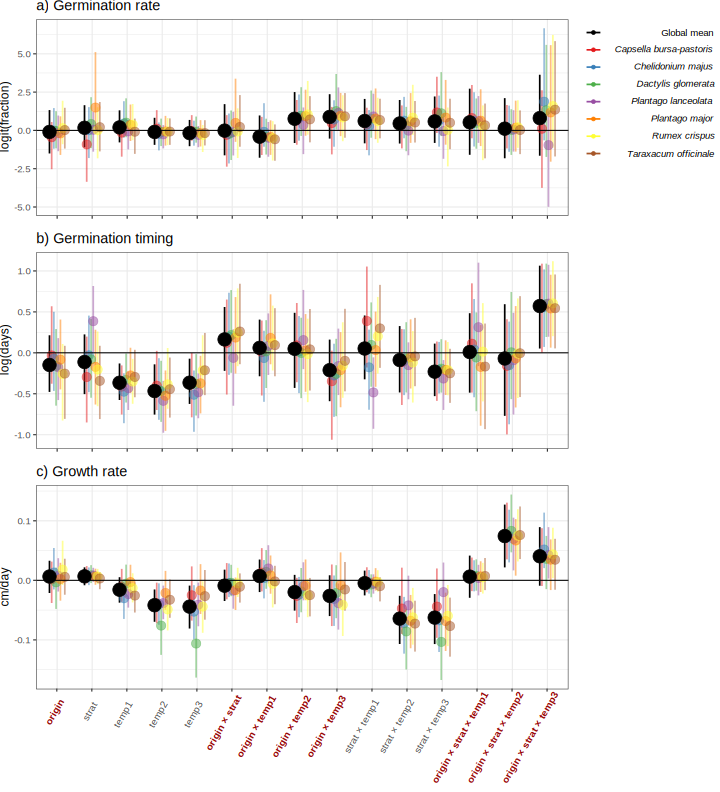
\includegraphics[scale=.5,angle=-90]{germ_figs_onepage.pdf}} %EMW-Mar2020: Perhaps we should have a raw data figure in the supp? Similar to what you have in your thesis?
	%HNE-Mar2020: Yes! I added to supp. not sure where to reference them? I went ahead and referenced them in results, but not sure if that's the best place? 
	\caption{Multilevel model coefficients with 95\% credible intervals, showing global average effects and species random effects. Intercept coefficients not shown.  a) model of germination rate, b) model of germination timing and c) model of growth rate}
	\label{fig:coef}
\end{figure}

	\section{Discussion} %EMW-Mar2020:  See comments in the comments file. 
	
	This study leveraged the power of a multi-species growth chamber experiments of native and introduced populations to investigate the importance of rapid evolution for invasive success. Across seven highly invasive plant species, we found only isolated support for the prevalence of post-introduction rapid evolution of key invasion traits of germination rate, timing, and growth rate. Instead, our results support the theory that these traits do not need to evolve for these species to invade: weediness, wide environmental tolerance, plasticity, or generalist traits in the source populations likely provide sufficient capacity to exploit novel environments \parencite{Baker1965}. Rapid evolution may provide a helping hand, but contrary to the many claims about the essentiality of rapid evolution in invasive species, it but may not be the dominant technique for invasion success, at least for these traits and these species. 
	
	These findings are  especially pronounced in germination rate, where all species germinated well and with scant sensitivity to climatic conditions, suggesting that the source populations of invading species provided invaders with the capacity to germinate in any environment, without the need to evolve. Some have suggested that while initially species may not need to evolve, they may once achieving a foot-hold \parencite{Lamarque2015}. However, many of the study species (e.g., DACGLO) have occupied their invasive range for centuries, yet still show little sign of an evolving germination response. 
	
	Overall, germination timing and growth rate did not show signs of post-invasion evolution. However, there was some evidence that particular responses have evolved: North American (invasive) populations appear to have evolved to germinate later and grow faster under high-temperature/long stratification combinations. Taking the climate of North American populations into account (Figure \ref{fig:sites}), this growth rate evolution may be adaptive. North American populations experience climates with longer winter stratification  (lower mean March temperatures) and hotter growing temperatures (higher mean May temperature). Thus, the capacity to grow faster at high temperatures after being exposed to our long stratification treatment may provide fitness advantages. Although it is  possible that these differences could be residual founder effects \parencite{Shirk2014}, a result of genetic drift \parencite{Eckert1996}, or that germination rate is not a fitness trait,  the convergence with experienced climate suggests that this observed change in growth rate is a sign of isolated adaptive evolution. 
	
	These results highlight the need to condition biological invasion mechanisms on specific invasion traits. Rapid evolution plays no role in germination rate, but does seem to play a limited role in growth rate. Rather than debating the overall importance of a specific mechanism, perhaps a better research direction lies in identifying what traits are likely to rapidly evolve to enable invasion, and which are not. Furthermore, the types of environmental variables that these traits evolve in response to can also be illuminating. Our results suggest that traits are most likely to evolve in response to specific combinations of spring temperature and winter length.  Adaptation to winter length is especially under-studied, and our results suggest that examining it is only useful in concert with other climate variables.  Not only can these trait evolution/environment relationships be useful for understanding invasions, they can also help delineate plant capacities to adapt to anthropogenic climate change.
	
	Our findings preliminarily suggest that these invasive species may be able to adapt to changing climates. Because cold-stratification is a simulation of temperate winter, the evidence that species can adapt their growth rate in accordance with winter length and spring temperature suggests that they may have the capacity to adapt to changing winter lengths and spring temperatures that anthropogenic climate change is bringing \parencite{IPCC2015}. These results also echo the  importance of varying both winter length and spring temperature in order to observe responses to climatic \parencite[e.g.,][]{Bernareggi2016}. 
	
	One weakness in our design is the limited number of individuals and populations collected from the invasive range (see Figure \ref{fig:sites}; Table \ref{tab:seeds}). This small geographic scale in the invasive range (North American) populations, could mean that our results are specific to New England, and not generalizable to other parts of the invasive range. It is possible that if we had included sampling sites from southern North America that we would see, for example,  rapid evolution of a higher growth rate at the highest temperature. However, the fact that our North American sampling sites do show substantial climate variation (Figure \ref{fig:sites}), suggests that our results do include a modicum of geographic variation in the invasive range. Furthermore, our Bayesian multilevel modeling framework enabled us to control for the greater sampling effort in the native range. 
 %EMW-Mar2020:  As I mentioned in comments file, I find these results super cool and think you should set the reader up a little more for them (and help them appreciate them). Basically, it suggests that if evolution on germination is happening, it might be complicated  -- more complicated than many designs test for. 
%HNE-Mar2020: Tried to address that in preceding paragraph. 
	
	Our study leveraged the capacity of growth chambers to study seven species simultaneously to eight climate treatments. However, this design does lack some of the real-world features of reciprocal common garden experiments, where realized climates exactly match the respective climates of the source populations. Common gardens also enable some degree of biotic interactions, which may often be important for determining invasions \parencite{Germain2018,Blois2013}.  Nevertheless, growth chambers provided a tractable design for testing multiple species from two continents in a precisely controlled experiment. Furthermore, while common garden experiments are fundamentally idiosyncratic and resource-intensive, future research could harness our growth chamber design and Bayesian modeling approach to test other invasive species, other populations, other traits, and other combinations of climate factors (including precipitation). Such future small-scale growth chamber studies could enable robust meta-analyses capable of identifying the traits and climate responses for which rapid evolution is, or is not, essential for invasion success. 
	

%EMW-Mar2020:  Somewhere in discussion mention benefits of growth chambers over common gardens, and mention benefits of common gardens over growth chambers -- and what next steps your results suggest someone should do.
%HNE-Mar2020: added above. 
As a rule, rapid evolution of germination and growth traits is not essential for invasion success. But rapid evolution may still play a role, especially in more extreme or different environments:  \textcite{Linde2001} found that CAPBUR evolved to colonize high-altitude and desert environments in California. However, we found little sign of evolution in our comparisons between temperate populations of this species. Perhaps, as suggested by Baker (1965), the generalist traits contained in temperate source populations are suitable as long as the introduced environment is not too different. Our findings provide support for  the speculation by van Kleunen and colleagues (2010) that future invasions can be predicted by species' characteristics, but perhaps only specific traits, such as germination rate. This finding suggests that managers can perhaps best guard against future invasions by targeting weedy species and preventing them from dispersing beyond their native ranges. 

	
\section{Acknowledgments}
This field work was supported by the Harvard College Research Fund and the Harvard University Center for the Environment Undergraduate Summer Research Fund. Thanks to E. Forrestel for mentorship to HNE. Thanks to J. Williams and H. Branch for fruitful discussions. Thanks also to D. Flynn, S. Gee, J. Samaha, and T. Savas for help transplanting, collecting, and measuring. Thanks to F. Rosin, K. Woodruff, and J. Gard for help with collection and growing logistics. Thanks to S. Fritz for help with data input. Thank you to M. Rucinski, C. Husic, N. Gilbert, A. Delgado, and A. Acosta for comments on earlier drafts of this paper. Thanks to J. Eyster, S. Stalhandske, and G. Barbone for assistance with and camaraderie during field sampling. 

	

\section{Literature Cited}
\printbibliography
\end{document}
